\appendix
\chapter{Appendix}

%----------------------------------------------------------------------------------------
%	Section
%----------------------------------------------------------------------------------------

\section{Feature Extraction}

\subsection{Shelving Filter Design}
\label{shelving-appendix}
For gain $G$ in dB, center frequency of transition band $F_c$ in Hz and sampling frequency $F_s$, coefficients of a high-frequency boost second-order shelving filter is calculated by following equations as described in \cite{DAFX_book}.

\begin{align}
\begin{split}
b_0 &= \frac{V_0 + \sqrt{2V_0} K + K^2}{1 + \sqrt{2} K + K^2}\\
b_1 &= \frac{2 (K^2 - V_0)}{1 + \sqrt{2} K + K^2}\\
b_2 &= \frac{V_0 - \sqrt{2V_0} K + K^2}{1 + \sqrt{2} K + K^2}\\
a_1 &= \frac{2 (K^2 - 1)}{1 + \sqrt{2} K + K^2}\\
a_2 &= \frac{1 - \sqrt{2}K + K^2}{1 + \sqrt{2}K + K^2}
\end{split}
\end{align}
where $a_0 = 1$, $K = \tan(\pi F_c / F_s)$ and $V_0 = 10^{G/20}$.

%--------------------------------------------
%--------------------------------------------

\subsection{Mel-frequency Cepstral Coefficients Extraction}
\begin{table}[H]
\centering
\caption{Frequency and Mel-scale Relationship}
\label{table:frequency-mel-relationship}
\begin{tabular}{rrr|rrr}
\toprule
m &$f[m]$ in Hz &Mel-scale in mel &m &$f[m]$ in Hz &Mel-scale in mel\\
0  & 0.0    & 0.0    & 11 & 1920.4 & 1485.0 \\
1  & 89.2   & 135.0  & 12 & 2254.5 & 1620.0 \\
2  & 189.9  & 270.0  & 13 & 2631.2 & 1755.0 \\
3  & 303.3  & 405.0  & 14 & 3055.9 & 1890.0 \\
4  & 431.3  & 540.0  & 15 & 3534.7 & 2025.0 \\
5  & 575.5  & 675.0  & 16 & 4074.7 & 2160.0 \\
6  & 738.1  & 810.0  & 17 & 4683.4 & 2295.0 \\
7  & 921.5  & 945.0  & 18 & 5369.8 & 2430.0 \\
8  & 1128.2 & 1080.0 & 19 & 6143.7 & 2565.0 \\
9  & 1361.3 & 1215.0 & 20 & 7016.2 & 2700.0 \\
10 & 1624.1 & 1350.0 & 21 & 8000.0 & 2835.0 \\
\bottomrule
\end{tabular}
\end{table}

%----------------------------------------------------------------------------------------
%	Section
%----------------------------------------------------------------------------------------

\section{Digital Signal Processor}

\subsection{Fixed-Point Data Types}

\begin{table}[H]
\centering
\caption{Fixed-Point Data Types}
\label{fixed-point-data-types}
\begin{tabu} to \textwidth {XXXX}
\toprule
Type &Size &Min &Max\\
\hline
\texttt{char} &8-bit &-128 &127\\
\hline
\texttt{unsigned char} &8-bit &0 &255\\
\hline
\texttt{short} &16-bit &-32,768 &32,767\\
\hline
\texttt{unsigned short} &16-bit &0 &65,535\\
\hline
\texttt{int} &32-bit &-2,147,483,648 &2,147,483,647\\
\hline
\texttt{unsigned int} &32-bit &0 &4,294,967,295\\
\hline
\texttt{long} &32-bit &-2,147,483,648 &2,147,483,647\\
\hline
\texttt{unsigned long} &32-bit &0 &4,294,967,295\\
\bottomrule
\end{tabu}
\end{table}

\subsection{Floating-Point Data Types}
\label{subsection:float-data-type}

\begin{figure}[H]
\begin{minipage}[t]{0.5\linewidth}
\centering
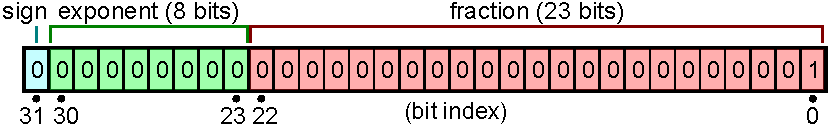
\includegraphics[width=\textwidth]{ang/smallest-denormalized-number}
\caption{Smallest Denormalized Number}
\label{ang/smallest-denormalized-number}
\end{minipage}
\begin{minipage}[t]{0.5\linewidth}
\centering
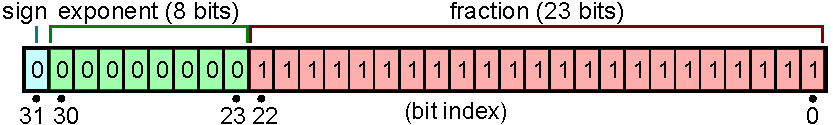
\includegraphics[width=\textwidth]{ang/largest-denormalized-number}
\caption{Largest Denormalized Number}
\label{ang/largest-denormalized-number}
\end{minipage}
\end{figure}

\begin{figure}[H]
\begin{minipage}[t]{0.5\linewidth}
\centering
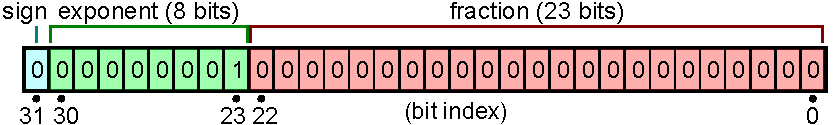
\includegraphics[width=\textwidth]{ang/smallest-normalized-number}
\caption{Smallest Normalized Number}
\label{ang/smallest-normalized-number}
\end{minipage}
\begin{minipage}[t]{0.5\linewidth}
\centering
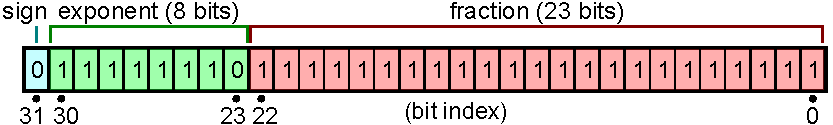
\includegraphics[width=\textwidth]{ang/largest-normalized-number}
\caption{Largest Normalized Number}
\label{ang/largest-normalized-number}
\end{minipage}
\end{figure}

Fig. \ref{ang/smallest-denormalized-number} to Fig. \ref{ang/largest-normalized-number} demonstrate the internal representation of a single-precision floating-point number. The actual mantissa (fraction part) includes 23 fraction bits to the right of the binary point and an \textit{implicit leading bit} to the left of the binary point. When the exponent part is equal to $(00000000)_2$, the implicit leading bit is with value 0 (denormalized); otherwise, the implicit leading bit takes 1 (normalized). Hence, the total length of mantissa is $(23 + 1)$ bits; in other words, \texttt{float} has a precision of $\log_{10}(2^{24}) \approx 7.225$ decimal digits.

\begin{align}
value &=
\begin{cases}
(-1)^{b_{31}} \times (0.b_{22}b_{21} \dots b_{0})_2 \times 2^{- 126} &\text{denormalized}\\
(-1)^{b_{31}} \times (1.b_{22}b_{21} \dots b_{0})_2 \times 2^{(b_{30}b_{29} \dots b_{23})_2 - 127} &\text{normalized}
\end{cases}\\
&=
\begin{cases}
\displaystyle(-1)^{b_{31}} \times \sum_{i=1}^{23} b_{23-i} 2^{-i} \times 2^{- 126} &\text{denormalized}\\
\displaystyle(-1)^{b_{31}} \times ( 1 + \sum_{i=1}^{23} b_{23-i} 2^{-i} ) \times 2^{\sum_{i=0}^{7} b_{i+23} 2^i - 127} &\text{normalized}
\end{cases}
\end{align}

\begin{table}[H]
\centering
\caption{Floating-Point Range}
\label{floating-point-range}
\begin{tabu} to \textwidth {XX}
\toprule
Number &Value\\
\hline
smallest denormalized number &$\pm 2^{-23} \times 2^{-126} \approx \pm 1.4 \times 10^{-45}$\\
\hline
largest denormalized number &$\pm (1-2^{-23}) \times 2^{-126} \approx \pm 1.18 \times 10^{-38}$\\
\hline
smallest normalized number &$\pm 1 \times 2^{-126} \approx \pm 1.18 \times 10^{-38}$\\
\hline
largest normalized number &$\pm (2-2^{-23}) \times 2^{127} \approx \pm 3.4 \times 10^{38}$\\
\bottomrule
\end{tabu}
\end{table}
